\documentclass[12pt]{article}

\usepackage{hyperref}
\usepackage{datetime}
\usepackage{graphicx}
\usepackage{minted}
\usepackage{caption}
\usepackage{amssymb}
\usepackage{float}
\usepackage[a4paper,width=150mm,top=25mm,bottom=25mm]{geometry}
\usepackage[utf8]{inputenc}

\hyphenpenalty=100000
\hypersetup{
    colorlinks=true,
    linkcolor=blue,
    filecolor=blue,      
    urlcolor=blue,
    unicode=false
}
\renewcommand*\contentsname{Tabelă de Conținut}
\renewcommand*\listfigurename{Listă de Imagini}
\renewcommand{\listtablename}{Listă de Tabele}
\captionsetup[table]{name=Tabel}
\renewcommand*\figurename{Imagine}
\usemintedstyle{bw}

\title{
    
\includegraphics[width=3cm, height=3.5cm]{Academy Logo.png} \\
    \vspace{5mm}
    {Specificarea Cerințelor Software pentru\\
    Proiectul \textbf{Aranea}}
    \vspace{10mm}
}
\vspace{20mm}
\author{
    Apostolescu Ștefan \\
    Băjan Ionuț-Mihăiță \\
    Brumă Ionuț-Cosmin \\
    Iosif George-Andrei \\
    Stanciu Răzvan-Daniel \\
    \vspace{10mm}
}
\ddmmyyyydate

\begin{document}

\null
\nointerlineskip 
\vfill
\let\snewpage \newpage
\let\newpage \relax
\maketitle
\let \newpage \snewpage
\vfill 
\break

\newpage

\tableofcontents

\newpage

\listoffigures

\listoftables

\newpage

\section{Detalii despre Document}

\subsection{Scop}
Scopul acestui document este de a descrie cu lux de amănunte modul în care membrii echipei, enumerați anterior, vor proiecta, implementa și testa sistemul Aranea pe baza cazurile de utilizare și a cerințele funcționale și nefuncționale.

\subsection{Conținut}
Documentul este împărțit în trei capitole. Primul oferă o descriere generală a proiectului, plecând de la problemele întâlnite și ajungând până la modul în care soluția dezvoltată le va rezolva. Al doilea capitol prezintă cerințele funcționale pe care proiectul trebuie să le îndeplinească, cuprinzând aici actorii implicați, limitele sistemului și cazurile de utilizare. Al treilea descrie cerințele nefuncționale, precum interfața cu utilizatorii, performanță, fiabilitate și securitate.

\newpage

\section{Descriere Generală a Proiectului}

\subsection{Situație Curentă}

Acum 25 de ani, numai 0.4\% din populația lumii era conectată la Internet. Datorită avantajelor evidente pe care acesta le oferă, numărul persoanelor care îl folosesc a crescut considerabil, în prezent fiind de peste 60\%\footnote{Conform  \href{https://www.internetworldstats.com/emarketing.htm}{Internet Growth Statistics}.}. \\
Această creștere s-a reflectat și în conținutul disponibil online. Deoarece devenise din ce în ce mai dificilă găsirea unei informații particulare, au fost introduse motoare software cu rolul de a căuta sistematic World Wide Web-ul. Acestea folosesc pentru indexarea informației un tip special de roboți, numit crawler sau spider. \\
Pe lângă acest caz de utilizare, un program de tip crawler mai este folosit pentru colectarea din World Wide Web a informațiilor care corespund anumitor criterii. De exemplu, o companie se poate folosi de un astfel de robot pentru a căuta pe Internet prețurile companiilor asemănătoare, din aceeași localitate, cu scopul de a obține un avantaj concurențial prin practicarea unor prețuri mai mici.

\subsection{Misiune}

Prin implementarea proiectul, se dorește oferirea unei soluții open-source pentru crawling web. Aceasta va putea fi folosită de către oricine, pentru a-și îndeplini sarcinile specifice, putând contribui în același timp la rezolvarea de erori, respectiv la dezvoltarea ulterioară a soluției, prin intermediul platformei \href{https://github.com/}{GitHub}.

\subsection{Context}

Aranea pune la dispoziția utilizatorilor, printr-o interfață în linie de comandă, o serie de operații utile descărcării locale a paginilor web și a procesării lor. \\
Crawling-ul constă în vizitarea recursivă a paginilor unor website-uri listate într-un fișier dat ca intrare programului. Printr-un alt fișier, de configurare, se va putea personaliza tot procesul de descărcare al paginilor. Acesta profită de puterea procesoarelor moderne, utilizând mai multe fire de execuție. Scopul final este de a salva local paginile care corespund anumitor criterii dictate de către utilizator și, opțional, de a genera hărți ale website-urilor. \\
Pe lângă crawling proiectul oferă posibilitatea de a filtra după o anumită extensie fișierele salvate local, de a căuta după un anumit șablon și de a solicita ajutor. \\
Soluția oferă avantajul de a fi rulată pe orice calculator. Nu necesită resurse superioare, însă, în cazul în care se dorește salvarea unui website publicat online (deci care nu aparține rețelei locale), este necesară o conexiune stabilă la Internet.

\subsection{Beneficii}

Beneficiile pe care proiectul le aduce constau, în primul rând, în funcționalitățile menționate anterior. Pe lângă acestea, mai oferă avantajele de a fi ușor de utilizat, open-source și de a nu necesita resurse superioare de la calculatorul pe care este rulat.

\newpage

\section{Cerințe Funcționale}

\subsection{Actori}

Actorii care interacționează cu sistemul sunt:
\begin{itemize}
    \item utilizatorul, care folosește soluția propusă, cu un set anume de date de intrare, pentru a-și îndeplini sarcinile specifice,
    \item server-ul web țintă, care găzduiește paginile ce se doresc a fi descărcate.
\end{itemize}

\subsection{Diagramă de Sistem}

\begin{center}
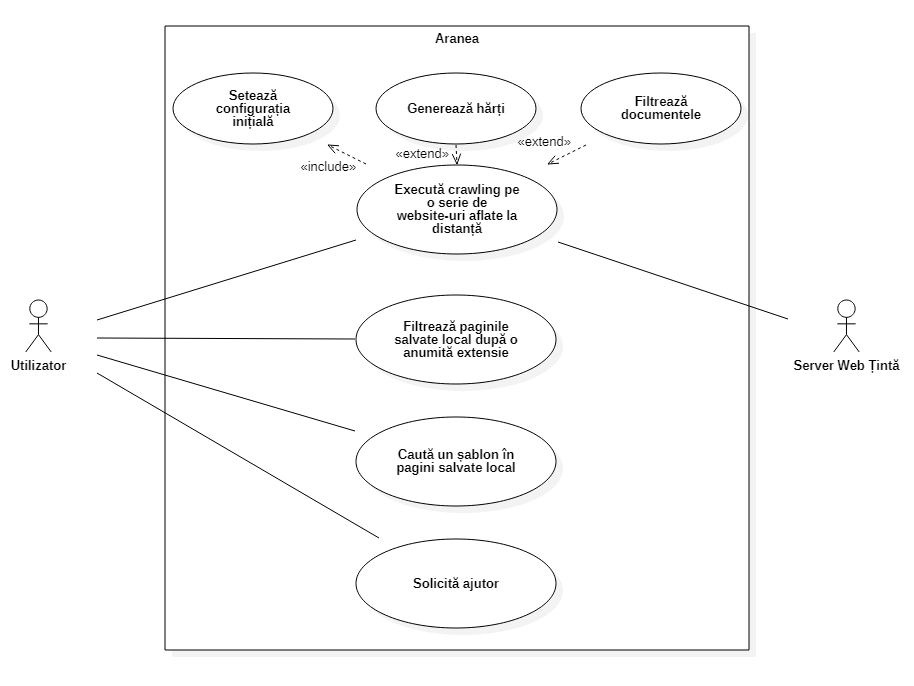
\includegraphics[width=15cm]{Use-case Diagram.png}
    \captionof{figure}{Diagramă de sistem}
\end{center}

\newpage

\subsection{Descrieri ale Cazurilor de Utilizare}

În tabelele următoare, pentru ușurarea folosirii soluției, au fost setate alias-urile menționate în secțiunea \hyperlink{interface_link}{cerințelor de interfață}. \\

\begin{table}[H]
    \centering
    \begin{tabular}{ |p{0.25\linewidth} | p{0.75\linewidth}| }
        \hline
        Caz de Utilizare & Execută crawling pe o serie de website-uri aflate la distanță \\
        Descriere Scurtă & Descarcă conținutului unor website-uri listate într-un fișier, pe baza unui alt fișier, de configurare.\\
        Prioritate & Ridicată \\
        Declanșator & Rularea comenzii \mintinline{bash}{aranea crawl URLS_FILE CONFIG_FILE} \\
        Condiții Inițiale & \begin{enumerate}
                                \item Existența fișierelor de intrare, cele date ca parametrii
                                \item Conexiune la Internet, în cazul în care acest lucru este necesar
                            \end{enumerate} \\
        Rută Uzuală & \begin{enumerate} 
                          \item Utilizatorul creează un fișier (\mintinline{bash}{URLS_FILE}) care conține referințe către website-uri ce trebuiesc descărcate.
                          \item Utilizatorul creează un fișier (\mintinline{bash}{CONFIG_FILE}) cu configurația operației.
                          \item Utilizatorul rulează comanda specifică, dând ca argumente fișierele menționate anterior.
                          \item Aranea efectuează operațiunea de crawling, pe mai multe fire de execuție, conform cu configurația primită.
                          \item Aranea salvează documentele descărcate în folder-ul menționat în fișierul de configurație.
                      \end{enumerate} \\
        Rute Alternative & \begin{enumerate}
                               \item Filtrarea conținutului descărcat
                               \item Crearea unor hărți
                           \end{enumerate} \\
        Condiții Ulterioare & Existența unui folder local ce conține documentele solicitate \\
        Excepții Posibile & \begin{enumerate}
                                \item Un server web țintă nu este disponibil.
                                \item Un website nu permite accesul, prin fișierul \mintinline{bash}{robots.txt}.
                                \item O pagină web referențiată nu există.
                                \item Nu se pot crea local foldere sau fișiere.
                            \end{enumerate} \\
        \hline
    \end{tabular}
    \caption{Descriere a cazului de utilizare pentru crawling}
    \label{table:1}
\end{table}

\newpage

\begin{table}[H]
    \centering
    \begin{tabular}{ |p{0.25\linewidth} | p{0.75\linewidth}| }
        \hline
        Caz de Utilizare & Setează configurația inițială \\
        Descriere Scurtă & Setează configurația folosită de Aranea, pe baza unui fișier local de configurare. \\
        Prioritate & Ridicată \\
        Declanșator & Specificarea parametrului \mintinline{bash}{CONFIG_FILE} în comanda \mintinline{bash}{aranea crawl URLS_FILE CONFIG_FILE} \\
        Condiții Inițiale & \varnothing \\
        Rută Uzuală & Utilizatorul specifică, într-un fișier local, următoarele elemente:
            \begin{itemize} 
                \item \mintinline{bash}{download_dir}, șir de caractere pentru directorul de descărcare
                \item \mintinline{bash}{log_file}, șir de caractere pentru fișierul de jurnal
                \item \mintinline{bash}{log_level}, întreg pentru prioritatea minimă a unui eveniment pentru a fi jurnalizat \textit{(opțional, implicit \mintinline{bash}{0})}
                \item \mintinline{bash}{is_sitemap_generated}, boolean care indică dacă se vor genera hărți pentru website-urile descărcate \textit{(opțional, implicit \mintinline{bash}{true})}
                \item \mintinline{bash}{max_threads}, întreg pentru numărul maxim de fire de execuție \textit{(opțional, implicit \mintinline{bash}{1000})}
                \item \mintinline{bash}{delay}, numărul de secunde între două cereri consecutive către un server web țintă \textit{(opțional, implicit \mintinline{bash}{1})}
                \item \mintinline{bash}{allowed_extensions}, șir de caractere pentru extensii ale fișierelor ce vor fi descărcate, separate prin virgulă \textit{(opțional, implicit \mintinline{bash}{*})}
                \item \mintinline{bash}{allowed_max_size}, întreg pentru dimensiunea maximă, în octeți, avută de un fișier ce va fi descărcat \textit{(opțional, implicit \mintinline{bash}{1000000000})}
                \item \mintinline{bash}{allowed_pattern}, șir de caractere pentru un șablon Regex ce trebuie să se regăsească într-un fișier pentru a fi descărcat \textit{(opțional, implicit \mintinline{bash}{""})}
                \item \mintinline{bash}{skip_robotsdottxt_files}, boolean care indică dacă fișierele menționate în \mintinline{bash}{robots.txt} nu vor fi descărcate \textit{(opțional, implicit \mintinline{bash}{true})}.
            \end{itemize} \\
        Rute Alternative & \varnothing \\
        Condiții Ulterioare & Existența unui fișier local, valid, de configurație \\
        Excepții Posibile & \begin{enumerate}
                                \item Formatul fișierului de configurare este invalid.
                                \item Fișierul de configurare nu conține toate câmpurile obligatorii.
                            \end{enumerate} \\
        \hline
    \end{tabular}
    \caption{Descriere a cazului de utilizare pentru setarea configurației inițiale}
    \label{table:1}
\end{table}

\begin{table}[H]
    \centering
    \begin{tabular}{ |p{0.25\linewidth} | p{0.75\linewidth}| }
        \hline
        Caz de Utilizare & Generează hărți \\
        Descriere Scurtă & Generează o hartă pentru fiecare website descărcat, aceasta listând toate fișierele componente. \\
        Prioritate & Medie \\
        Declanșator & Setarea câmpului \mintinline{bash}{is_sitemap_generated} din fișierul de configurare \\
        Condiții Inițiale & Finalizarea descărcării website-ului curent \\
        Rută Uzuală & După finalizarea fiecărei descărcări a unui website, Aranea parcurge folder-ul specific lui și listează toate fișierele într-un alt fișier de tip hartă.\\
        Rute Alternative & \varnothing \\
        Condiții Ulterioare & Existența unor fișiere locale, reprezentând hărțile \\
        Excepții Posibile & \begin{enumerate}
                                \item Folder-ul nu conține niciun fișier.
                            \end{enumerate} \\
        \hline
    \end{tabular}
    \caption{Descriere a cazului de utilizare pentru generarea hărților}
    \label{table:1}
\end{table}

\newpage

\begin{table}[H]
    \centering
    \begin{tabular}{ |p{0.25\linewidth} | p{0.75\linewidth}| }
        \hline
        Caz de Utilizare & Filtrează documentele \\
        Descriere Scurtă & Înainte de a descărca un fișier de pe server-ul web țintă, verifică dacă el corespunde anumitor criterii setate de către utilizator. \\
        Prioritate & Medie \\
        Declanșator & Setarea a cel puțin unul din câmpurile următoare, din fișierul de configurare: 
            \begin{itemize}
                \item \mintinline{bash}{allowed_extensions}
                \item \mintinline{bash}{allowed_max_size}
                \item \mintinline{bash}{allowed_pattern}
                \item \mintinline{bash}{skip_robotsdottxt_files}.
            \end{itemize} \\
        Condiții Inițiale & \varnothing \\
        Rută Uzuală & Pentru fiecare fișier ce se descoperă pe website-ul curent, Aranea verifică următoarele: 
            \begin{itemize}
                \item dacă \mintinline{bash}{allowed_extensions} este setat și dacă extensia fișierului apare în \mintinline{bash}{allowed_extensions}
                \item dacă \mintinline{bash}{allowed_max_size} este setat și dacă dimensiunea fișierului este mai mică decât \mintinline{bash}{allowed_max_size}
                \item dacă \mintinline{bash}{allowed_pattern} este setat și dacă apar în fișier șiruri de caractere care potrivesc \mintinline{bash}{allowed_pattern}
                \item dacă \mintinline{bash}{skip_robotsdottxt_files} este setat și dacă fișierul curent nu apare în \mintinline{bash}{robots.txt}.
            \end{itemize} \\
        Rute Alternative & \varnothing \\
        Condiții Ulterioare & Permisiunea descărcării unui fișier anume \\
        Excepții Posibile & \varnothing \\
        \hline
    \end{tabular}
    \caption{Descriere a cazului de utilizare pentru filtrarea documentelor}
    \label{table:1}
\end{table}

\newpage

\begin{table}[H]
    \centering
    \begin{tabular}{ |p{0.25\linewidth} | p{0.75\linewidth}| }
        \hline
        Caz de Utilizare & Filtrează paginile salvate local după o anumită extensie \\
        Descriere Scurtă & Filtrează paginile salvate local, aparținând unor website-uri, după extensie \\
        Prioritate & Ridicată \\
        Declanșator & Rularea comenzii \mintinline{bash}{aranea list EXTENSION} \\
        Condiții Inițiale & \varnothing \\
        Rută Uzuală & Aranea parcurge directoarele specifice unor website-uri, listând în linie de comandă fișierele cu o anumită extensie.\\
        Rute Alternative & \varnothing \\
        Condiții Ulterioare & Afișarea listării solicitate, în linie de comandă \\
        Excepții Posibile & \varnothing \\
        \hline
    \end{tabular}
    \caption{Descriere a cazului de utilizare pentru filtrarea după o anumită extensie a paginilor salvate local}
    \label{table:1}
\end{table}

\newpage

\begin{table}[H]
    \centering
    \begin{tabular}{ |p{0.25\linewidth} | p{0.75\linewidth}| }
        \hline
        Caz de Utilizare & Caută un șablon în pagini salvate local \\
        Descriere Scurtă & Caută un șablon în paginile descărcate local, aparținând unor website-uri. \\
        Prioritate & Ridicată \\
        Declanșator & Rularea comenzii \mintinline{bash}{aranea search PATTERN} \\
        Condiții Inițiale & Existența a cel puțin un folder care să reprezinte un website descărcat anterior \\
        Rută Uzuală & Aranea caută recursiv în toate directoarele, printând în linie de comandă numele fișierelor care conțin șiruri de caractere ce potrivesc șablonul.\\
        Rute Alternative & \varnothing \\
        Condiții Ulterioare & Afișarea în linie de comandă a fișierelor găsite \\
        Excepții Posibile & \begin{enumerate}
                                \item Folder-ul de descărcări este gol.
                            \end{enumerate} \\
        \hline
    \end{tabular}
    \caption{Descriere a cazului de utilizare pentru căutarea unui șablon în paginile salvate local}
    \label{table:1}
\end{table}

\newpage

\begin{table}[H]
    \centering
    \begin{tabular}{ |p{0.25\linewidth} | p{0.75\linewidth}| }
        \hline
        Caz de Utilizare & Solicită ajutor \\
        Descriere Scurtă & Solicită ajutorul cu privire la utilizarea programului. \\
        Prioritate & Medie \\
        Declanșator & Rularea comenzilor \mintinline{bash}{aranea} sau \mintinline{bash}{aranea help} \\
        Condiții Inițiale & \varnothing \\
        Rută Uzuală & Aranea afișează în linie de comandă o detaliere a folosirii programului\\
        Rute Alternative & \varnothing \\
        Condiții Ulterioare & Afișarea în linie de comandă a unei detalierii menționate anterior\\
        Excepții Posibile & \varnothing \\
        \hline
    \end{tabular}
    \caption{Descriere a cazului de utilizare pentru solicitarea ajutorului}
    \label{table:1}
\end{table}

\newpage

\section{Cerințe Nefuncționale}

\hypertarget{interface_link}{\subsection{Cerințe de Interfață}}

Proiectul va putea rula pe calculatoare cu sisteme de operare moderne (Windows, Linux și macOS), dotate cu Java Virtual Machine. O conexiune la Internet este necesară în cazul în care se doresc accesate website-uri din afara rețelei locale. \\
Interfața proiectului va fi în linie de comandă. Utilizarea va necesita cunoștințe minime de operare a unui calculator, aceasta fiind ușurată de aspecte precum:
\begin{itemize}
    \item posibilitatea setării unor alias-uri cu ajutorul comenzilor \\ \mintinline{bash}{doskey aranea=java -jar ABSOLUTE_PATH_TO/aranea.jar} pe Windows și \mintinline{bash}{alias aranea=java -jar ABSOLUTE_PATH_TO/aranea.jar} pe Linux și macOS
    \item comenzi simple, ușor de memorat
    \item acces la o detaliere a utilizării proiectului, cu ajutorul comenzilor \mintinline{bash}{aranea} sau \mintinline{bash}{aranea help}. 
\end{itemize}

\subsection{Cerințe de Performanță}

Aranea, fiind un proiect software simplu, nu necesită dotări suplimentare pe lângă cele solicitate de Java Virtual Machine. Prin implementarea ce favorizează folosirea de fire de execuție, garantează o performanță ridicată, ce poate fi însă scăzută de viteza sau de instabilitatea conexiunilor cu website-urile țintă.

\subsection{Cerințe de Securitate}

Cum unele website-uri sunt protejate de firewall-uri, există riscul ca adresa utilizatorului să fie blocată. Astfel, accesul de pe aceasta nu ar fi permis, chiar dacă ar fi vorba de navigarea neautomată (din browser) a website-ului. \\
Pentru a micșora acest risc, toate cererile către serverele web sunt distanțate implicit de o secundă și identificate printr-un agent specific, \mintinline{bash}{AraneaBot}.

\end{document}